\documentclass[11pt]{article}
\usepackage[letterpaper,margin=1in]{geometry}
\usepackage{amsmath,amssymb,amsthm}
\usepackage{tikz}
\usetikzlibrary{arrows.meta,calc}
\usepackage{xcolor}
\usepackage[hidelinks]{hyperref}
\hypersetup{pdftitle={Triangular and pentagonal chains},pdfauthor={Vamshi Jandhyala}}
\setlength{\parskip}{0.4em}
\setlength{\parindent}{0pt}

\newtheorem{theorem}{Theorem}
\newtheorem{lemma}[theorem]{Lemma}
\newtheorem{proposition}[theorem]{Proposition}
\theoremstyle{definition}
\newtheorem{definition}[theorem]{Definition}
\theoremstyle{remark}
\newtheorem*{remark}{Remark}
\newtheorem*{example}{Example}

\definecolor{inkblue}{RGB}{40,76,105}
\definecolor{softblue}{RGB}{226,235,243}
\definecolor{rust}{RGB}{153,70,45}
\definecolor{softrust}{RGB}{246,226,205}

\newcommand{\blk}[2]{B^{#2}_{#1}}


\title{Triangular and pentagonal chains}
\author{Vamshi Jandhyala}
\date{}

\begin{document}
\maketitle
\vspace{-2em}

\begin{abstract}
Can the numbers $1,2,\dots,n$ be written in a row so that every two neighbors add up to a
triangular number? Berlekamp and Guy observed that this is possible for $n=2$ and for every $n$
from $9$ to $70$, and that a closed loop with the same property exists for $12\le n\le 70$
except $n=14$. They asked for proofs. We prove both statements for every $n$, and also their conjecture
for generalized pentagonal numbers: chains for all $n\ge4$ and closed loops for all $n\ge9$. The proof
inflates a chain on $1,\dots,n$ to a chain on about $49n$ numbers, using the identity
$49T_k+6=T_{7k+3}$, and stitches $49$ inflated copies together with the numbers $1,\dots,27$.
The method is the one Gerbicz used for perfect squares; for triangular numbers it becomes
simpler, because every number can be kept in a position of its own parity. The stitching patterns and the starting cases are finite computations, checked independently;
the inductive existence argument is checked in the Lean proof assistant, with the starting cases as a
hypothesis.
\end{abstract}

\section{The question}

Try this before reading on: write $1,2,\dots,9$ in a row so that each pair of neighbors sums to
one of the triangular numbers
\[
  T_k=\tfrac{k(k+1)}{2}\colon\qquad 1,\ 3,\ 6,\ 10,\ 15,\ 21,\ 28,\ 36,\ \dots
\]
One answer is
\[
  3,\ 7,\ 8,\ 2,\ 4,\ 6,\ 9,\ 1,\ 5,
\]
whose neighbor sums are $10,15,10,6,10,15,10,6$. With eight numbers it cannot be done, and the
same holds for every $n$ from $3$ to $8$; a short search confirms it. Call such an arrangement a
\emph{triangular chain} of length $n$. If in addition the last and first numbers sum to a
triangular number, so that the row closes into a loop, call it a \emph{triangular necklace}.
Figure~\ref{fig:necklace} shows one for $n=12$.

\begin{figure}[ht]
\centering
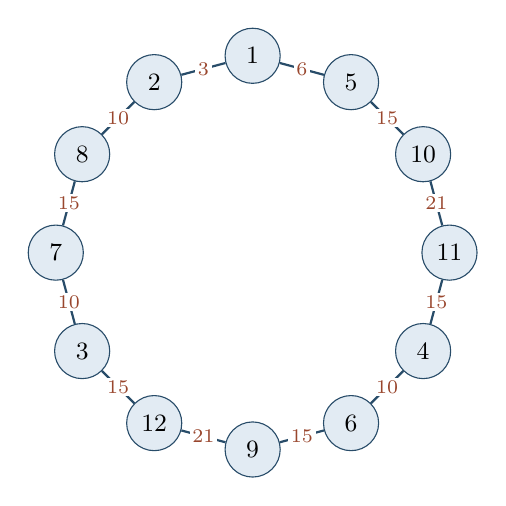
\begin{tikzpicture}[scale=1.25]
  \foreach \v [count=\i from 0] in {1,5,10,11,4,6,9,12,3,7,8,2} {
    \node[circle,draw=inkblue,fill=softblue,minimum size=7mm,inner sep=0pt]
      (n\i) at ({90-30*\i}:2) {\small $\v$};
  }
  \foreach \i/\s in {0/6,1/15,2/21,3/15,4/10,5/15,6/21,7/15,8/10,9/15,10/10,11/3} {
    \pgfmathtruncatemacro{\j}{mod(\i+1,12)}
    \draw[inkblue,thick] (n\i) -- (n\j)
      node[midway,font=\scriptsize,text=rust,fill=white,inner sep=1pt] {$\s$};
  }
\end{tikzpicture}
\caption{A triangular necklace of length $12$. Each bead is a number, and each link is labeled
with the triangular number its two beads add up to.}
\label{fig:necklace}
\end{figure}

The question comes from a paper of Berlekamp and Guy \cite{BG}, written in 2003 and printed in
2020, about chains whose adjacent sums lie in a prescribed set: squares, cubes, triangular and
pentagonal numbers, Fibonacci numbers. For the Fibonacci numbers they determine exactly which $n$ admit a chain \cite[Theorem~1]{BG}. For
triangular numbers they write that chains exist for $n=2$ and probably for all $n\ge 9$, that
necklaces appear to exist for all $n\ge12$ except $n=14$, and that they ``would like to see proofs
of these statements, which we have verified to $n=70$'' \cite[p.~343]{BG}. The square case,
popularized as the ``square-sum problem'', was settled by Gerbicz in 2018 in a computer-assisted
argument posted online \cite{Gerbicz,A090461}; a 2020 survey of Guy's number theory records that,
apart from squares, ``all other cases remain wide open'' \cite{JW}. For triangular sums the
numbers of chains are tabulated to $n=35$ in the OEIS \cite{A116980}, and a 2021 programming
contest asked for necklaces for every $n\le200$ \cite{topcoder}; to our knowledge no argument for all $n$ was known.
Neighboring questions have their own literature: splitting $1,\dots,2n$ into pairs with square sums
\cite{HKP}, and necklaces of $0,1,\dots,n-1$ in which neighbors differ by one of two given values \cite{WGS}.
For prime sums, circles on $1,\dots,2n$ are now known to exist for every large $n$ \cite{She}; that
proof uses perfect matchings and robust expansion, which need far more edges than the graphs met below.

\begin{theorem}\label{thm:main}
For $n\ge2$, a triangular chain of length $n$ exists exactly when $n=2$ or $n\ge 9$. A triangular necklace of
length $n\ge3$ exists exactly when $n\ge 12$ and $n\ne 14$.
\end{theorem}

The same holds one step up. Berlekamp and Guy also report that chains whose adjacent sums are
generalized pentagonal numbers $P_k=k(3k-1)/2$, $k\in\mathbb Z$ (that is, $1,2,5,7,12,15,22,26,\dots$),
appear to exist for all $n\ge4$, and necklaces for all $n\ge9$, checked to $n=49$ \cite[pp.~344--345]{BG}.

\begin{theorem}\label{thm:pent}
For $n\ge2$, a pentagonal chain of length $n$ exists exactly when $n\ge4$. A pentagonal necklace of
length $n\ge3$ exists exactly when $n\ge9$.
\end{theorem}

The ``only when'' halves concern finitely many $n$ and are settled by exhaustive search. The work
is in the other halves, which are statements about every $n$.

Why is this hard? Think of the numbers $1,\dots,n$ as the vertices of a graph, joined when their
sum is triangular; a chain is then a Hamiltonian path. Only about $2\sqrt n$ triangular numbers lie below $2n$,
so each vertex has at most that many neighbors, and the graph is far too sparse for the general
theorems that guarantee Hamiltonian paths in dense graphs. Searching
works for any given $n$ but proves nothing about all of them. What is needed is a way to build
long chains out of short ones.

\section{A first construction: billiards}

Berlekamp and Guy found many large necklaces by a construction they describe in terms of a
billiard table \cite[p.~343]{BG}. It shows what the sums can do in the simplest setting, so we start there.

Fix a triangular number $A$. The map $x\mapsto A-x$ reverses the interval $[1,A-1]$ and pairs
each $x$ in it with a partner, such that the pair sums to $A$. If $A$ is odd nothing is paired with
itself. A second reflection $x\mapsto C-x$ does the same on another interval. Now take two
odd triangular numbers $A<C$, set $n=C-A$, and assume $A\le n+1$. Every $x\in[1,n]$ has exactly one
partner among $A-x$ and $C-x$ in $[1,n]$: the first if $x<A$, the second if $x\ge A$. (Without
the assumption this fails: for $A=15$, $C=21$, $n=6$, the number $1$ has no partner.) So the two reflections
together form a perfect matching $M_{AC}$ of $[1,n]$ by triangular sums. A second pair $B<D$ of
odd triangular numbers with the same difference $D-B=n$ gives a second matching $M_{BD}$, provided
$B\le n+1$, which keeps every partner $B-x$ or $D-x$ inside $[1,n]$.

\begin{proposition}\label{prop:billiard}
Let $A<B<C<D$ be odd triangular numbers with $A+D=B+C$, put $n=C-A$, and assume $B\le n+1$.
(so also $A<B\le n+1$). Then $M_{AC}\cup M_{BD}$ is a triangular necklace on $[1,n]$ if and only if $\gcd(B-A,n)=2$.
\end{proposition}

\begin{proof}
Every vertex has one edge from each matching, so $M_{AC}\cup M_{BD}$ is a union of cycles that
alternate between the two matchings. Follow two steps, first $M_{AC}$ and then $M_{BD}$. The
composition of the reflections $x\mapsto S-x$ and $x\mapsto S'-x$ is $x\mapsto x+(S'-S)$, and here
$S\in\{A,C\}$ and $S'\in\{B,D\}$. Since $C\equiv A$ and $D\equiv B$ modulo $n$, every such step is
the rotation $x\mapsto x+(B-A)$ of $\mathbb Z/n$. A cycle of length $2\ell$ alternates between two
orbits of this rotation, each of size $\ell$, and the rotation has $\gcd(B-A,n)$ orbits. So there is
a single cycle, through all $n$ vertices, exactly when $\gcd(B-A,n)=2$.
\end{proof}

The eight smallest necklaces this produces have $n=90,198,234,450,540,550,650,782$; they are the
first eight rows of the table in \cite{BG}, which starts from $(A,B,C,D)=(1,15,91,105)$. But the
proposition needs $n$ to be a difference of two triangular numbers in two different ways, both
with a small subtrahend, and most $n$ are not. Billiards give infinitely many necklaces, never all
of them.

\section{Inflating a chain}

The identity behind everything else is
\begin{equation}\label{eq:inflate}
  49\,T_k+6=T_{7k+3},
\end{equation}
which says, after doubling, that $49k(k+1)+12=(7k+3)(7k+4)$. It is classical: it appears, with its
generalization below, in a 1974 survey of Hoggatt and Bicknell \cite[(4.3), (4.5)]{HB}. What is new
here is its use. Read it as a rule for numbers whose
sum is triangular: if $a+b=T_k$, then $(49a+c)+(49b+6-c)=T_{7k+3}$ for any integer $c$. So
multiplying by $49$ and shifting by $c$ and $6-c$ in turn keeps sums triangular.

To make the shifts alternate automatically we restrict to sums that are \emph{odd} triangular
numbers. If $a+b$ is odd then one of $a,b$ is odd and the other is even, so define
\[
  f_c(v)=\begin{cases} 49v+c & v \text{ odd},\\ 49v+6-c & v\text{ even}.\end{cases}
\]

\begin{example}
The chain $1,2$ has sum $3=T_2$. Its image under $f_c$ is $49+c,\ 104-c$, with sum $153=T_{17}$.
\end{example}

\begin{lemma}\label{lem:block}
If $a+b$ is an odd triangular number, then so is $f_c(a)+f_c(b)$. Consequently $f_c$ maps a chain
whose adjacent sums are odd triangular numbers to another such chain.
\end{lemma}

\begin{proof}
One of $a,b$ is odd and the other even, so $f_c(a)+f_c(b)=49(a+b)+6$, which is triangular by
\eqref{eq:inflate}, and odd because $a+b$ is.
\end{proof}

The constant $49$ is the smallest that works this way. In general
$(2m+1)^2T_k+T_m=T_{(2m+1)k+m}$, and we need the shift $T_m$ to be even, so that $c$ and $T_m-c$
can be equal ($c=3$ for $m=3$). That fixed offset turns out to be essential in Section~5.

\section{Chains that respect parity}

In a chain all of whose adjacent sums are odd, odd and even numbers alternate. If such a chain of
length $N$ starts with an odd number, then every number $v$ sits at a position of the same parity
as $v$. We work only with chains of this kind.

Why insist on parity? In the inflation step below, a chain $s$ of length $n$ and a chain
$t$ of length $n+1$ are both inflated, and the pieces must fit together without collisions. With
parity built in, each number has the same position parity in $s$ as in $t$, automatically. Gerbicz
needed an extra compatibility condition between the chains of lengths $n$ and $n+1$ (a ``nice
pair'', in his words \cite{Gerbicz}); parity makes it unnecessary. It is also close to forced: if a single rule assigned each number a position
parity valid in chains of every length $N\ge N_0$, then the number of odd positions, $\lceil N/2\rceil$,
grows with $N$ exactly when $N$ is odd, so every number $N>N_0$ would occupy a position of its
own parity.

We also fix the two ends of each chain, for a reason that will appear in Section~6.

\begin{definition}
For $N\ge2$ let $e(N)=2$ if $N$ is even and $e(N)=9$ if $N$ is odd. A \emph{good chain} of length
$N$ is an arrangement of $1,\dots,N$ that starts at $1$, ends at $e(N)$, and in which every two
neighbors sum to an odd triangular number.
\end{definition}

Since $1+2=3$ and $1+9=10$ are triangular, a good chain is also a necklace. For example $1,2$ is a
good chain of length $2$. The next lengths for which our searches found good chains are $54$ and
every larger length we tried.

\section{Covering $[28,N]$ by inflated chains}

Let $N=49n+r$ with $28\le r\le 76$ and $n\ge1$, and suppose $s$ and $t$ are good chains of lengths
$n$ and $n+1$. For each offset $c$ in the window $-21\le c\le 27$ we will use one \emph{block}
\[
  \blk{c}{s}=f_c(s)\quad\text{or}\quad \blk{c}{t}=f_c(t),
\]
meaning the chain $s$ or $t$ with $f_c$ applied to each entry. Both offsets $c$ and $6-c$ lie in the
window, so every entry of a block has the form $49v+o$ with $v\ge1$ and $-21\le o\le27$. These
$49$ consecutive offsets mean that an entry determines both $v$ and $o$, and that every block entry
is at least $49-21=28$. The numbers $1,\dots,27$ are left over; we call them \emph{glue}.

Which chain should block $c$ use? Its entries are $f_c(v)$ for $v$ up to the length of its chain,
and only $v=n+1$ can exceed $N$. That top entry is $49(n+1)+o_c$, where $o_c=c$ if $n+1$ is odd and
$o_c=6-c$ if $n+1$ is even. So block $c$ may use $t$ exactly when $o_c\le r-49$, and we let it do so
then. Figure~\ref{fig:grid} shows the picture.

\begin{figure}[ht]
\centering
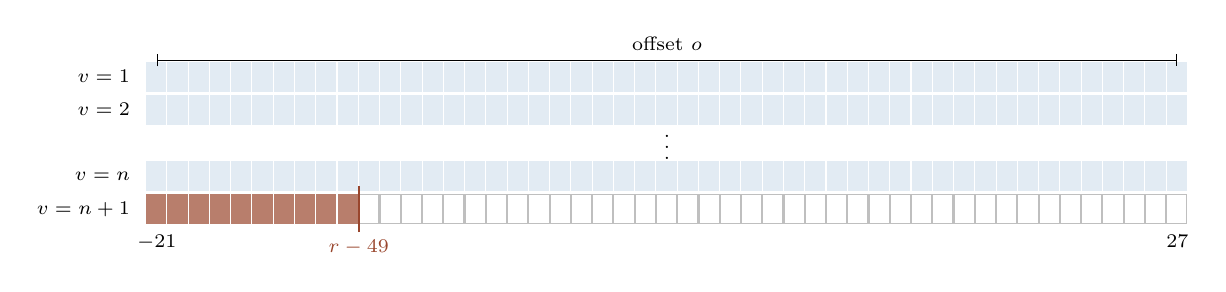
\begin{tikzpicture}[x=0.27cm,y=0.42cm]
  % rows: v = 1, 2, 3, ..., n, n+1 ; columns: offset o = -21..27
  \foreach \row/\lab in {0/{v=n+1},1/{v=n},3/{v=2},4/{v=1}} {
    \node[left,font=\scriptsize] at (-21.8,\row+0.5) {$\lab$};
  }
  \node[font=\scriptsize] at (3,2.6) {$\vdots$};
  \foreach \row in {1,3,4} {
    \foreach \o in {-21,...,27} { \fill[softblue] (\o-0.5,\row+0.05) rectangle (\o+0.45,\row+0.95); }
  }
  \foreach \o in {-21,...,27} {
    \pgfmathparse{\o<=-12 ? 1 : 0}
    \ifnum\pgfmathresult=1
      \fill[rust!70] (\o-0.5,0.05) rectangle (\o+0.45,0.95);
    \else
      \draw[gray!50] (\o-0.5,0.05) rectangle (\o+0.45,0.95);
    \fi
  }
  \draw[thick,rust] (-11.5,-0.2) -- (-11.5,1.2);
  \node[below,font=\scriptsize] at (-21,0) {$-21$};
  \node[below,font=\scriptsize] at (27,0) {$27$};
  \node[below,font=\scriptsize,text=rust] at (-11.5,-0.15) {$r-49$};
  \node[above,font=\scriptsize] at (3,5.0) {offset $o$};
  \draw[|-|] (-21,5) -- (27,5);
\end{tikzpicture}
\caption{The number $49v+o$ sits in row $v$ and column $o$; every integer from $28$ up has exactly
one cell. Rows $1,\dots,n$ (blue) are filled by the blocks whatever chains they use. In row $n+1$
only the cells with $o\le r-49$ are at most $N$ (shown here for $r=37$); these are the top entries
of the blocks that use $t$.}
\label{fig:grid}
\end{figure}

\begin{lemma}\label{lem:cover}
With this choice, the $49$ blocks together with the glue numbers $1,\dots,27$ contain every integer
from $1$ to $N$ exactly once.
\end{lemma}

\begin{proof}
Within one block the entries are distinct, since an entry determines $v$. Two different blocks
$c\ne c'$ never share an entry: $f_c(v)=f_{c'}(v')$ forces $v=v'$ and then equal offsets, but the
offsets of $f_c(v)$ and $f_{c'}(v)$ are $c$ and $c'$ when $v$ is odd, and $6-c$ and $6-c'$ when $v$
is even. Glue numbers are below $28$, block entries are not. Every entry is at most $N$: entries
with $v\le n$ are at most $49n+27<N$, and an entry with $v=n+1$ belongs to a block using $t$, whose
top entry is at most $49(n+1)+r-49=N$ by the choice. Finally count. The map $c\mapsto o_c$ permutes
the window, so exactly $(r-49)-(-21)+1=r-27$ blocks use $t$, and the total number of entries is
$27+49n+(r-27)=N$. Distinct integers in $[1,N]$, $N$ of them, are all of $[1,N]$.
\end{proof}

The proof is just counting, and it does not use the parity of positions at all. Parity is needed
in the next step, where the blocks are joined.

\section{Stitching}

Lemma~\ref{lem:cover} gives $76$ pieces: $27$ single glue numbers and $49$ blocks, each a chain
with odd triangular adjacent sums (Lemma~\ref{lem:block}). It remains to put them in a row, each
block read forwards or backwards, so that every junction is also an odd triangular sum, the row
starts at $1$, and it ends at $e(N)$. Then the row is a good chain of length $N$.

Here is the point that makes this a finite problem. A block's two ends do not depend on $n$
beyond its parity. Because $s$ and $t$ start at $1$ and end at $2$ or $9$, block $c$ starts at
$f_c(1)=49+c$ and ends at $f_c(2)=104-c$ or $f_c(9)=441+c$, according to the parity of the
length of its chain. Which blocks use $t$ depends on $r$ and on the parity of $n$. So the
stitching problem has only $49\times2=98$ versions, one for each $r\in[28,76]$ and each parity of
$n$, and a solution of one version serves every $n$ of that parity.

\begin{proposition}\label{prop:step}
For each $r\in[28,76]$ and each parity of $n$ there is an ordering and orientation of the $76$
pieces with all junction sums odd triangular, starting at $1$ and ending at $e(49n+r)$.
Consequently, if good chains of lengths $n$ and $n+1$ exist, so does a good chain of length
$49n+r$.
\end{proposition}

\begin{proof}
The second sentence follows from the first and Lemmas~\ref{lem:block} and~\ref{lem:cover}. The first is
a finite statement, one arrangement for each of the $98$ cases; we list them all in the data
accompanying this paper, and each was checked as described in Section~\ref{sec:checks}.
\end{proof}

We found the $98$ arrangements with a constraint solver: Google's CP-SAT \cite{ortools}, whose
circuit constraint expresses a Hamiltonian path directly. All $98$ took under two seconds in total.
To give the flavor, here is the arrangement for $r=28$ and $n$ even, writing $\blk{c}{s}$ for a
block read forwards and $\overleftarrow{\blk{c}{s}}$ for one read backwards; glue numbers appear
as themselves.
\begin{quote}\small\raggedright
$1$, $\blk{-5}{s}$, $\overleftarrow{\blk{-18}{s}}$, $24$, $21$, $\overleftarrow{\blk{20}{s}}$, $22$, $23,\
\overleftarrow{\blk{22}{s}}$, $\overleftarrow{\blk{4}{s}}$, $\blk{3}{s}$, $\blk{21}{s},\
\overleftarrow{\blk{16}{s}}$, $\overleftarrow{\blk{-2}{s}}$, $\blk{9}{s}$, $10$, $5$, $\blk{-9}{s},\
\overleftarrow{\blk{-14}{s}}$, $20$, $25$, $\overleftarrow{\blk{24}{s}}$, $18,\
\overleftarrow{\blk{17}{s}}$, $\overleftarrow{\blk{-1}{s}}$, $\overleftarrow{\blk{-19}{s}}$, $15,\
\overleftarrow{\blk{-21}{t}}$, $27$, $\blk{15}{s}$, $16$, $\blk{-10}{s}$, $\blk{8}{s}$, $\blk{26}{s},\
\overleftarrow{\blk{11}{s}}$, $\blk{-4}{s}$, $\blk{14}{s}$, $\overleftarrow{\blk{23}{s}},\
\overleftarrow{\blk{5}{s}}$, $\overleftarrow{\blk{-13}{s}}$, $19$, $26$, $\overleftarrow{\blk{25}{s}},\
17$, $\blk{-11}{s}$, $\blk{7}{s}$, $8$, $7$, $\overleftarrow{\blk{6}{s}}$, $\overleftarrow{\blk{-12}{s}},\
\blk{19}{s}$, $\overleftarrow{\blk{18}{s}}$, $\overleftarrow{\blk{0}{s}}$, $6$, $9$, $12,\
\blk{-16}{s}$, $\overleftarrow{\blk{-7}{s}}$, $3$, $\overleftarrow{\blk{2}{s}}$, $4$, $\blk{-8}{s},\
\overleftarrow{\blk{-15}{s}}$, $11$, $\overleftarrow{\blk{10}{s}}$, $\blk{-3}{s},\
\overleftarrow{\blk{-20}{s}}$, $\blk{27}{s}$, $14$, $\overleftarrow{\blk{13}{s}}$, $\blk{-6}{s},\
\blk{12}{s}$, $13$, $\blk{-17}{s}$, $\blk{1}{s}$, $2$.
\end{quote}
For $r=28$ only block $-21$ uses $t$. Since $n$ is even, $s$ ends at $2$, so $\blk{c}{s}$ runs
from $49+c$ to $f_c(2)=104-c$. The first three junctions are $1+44=45=T_9$, then $109+122=231=T_{21}$
(the end of $\blk{-5}{s}$ meets the start of $\overleftarrow{\blk{-18}{s}}$, which is $104+18$), then
$31+24=55=T_{10}$ (the reversed block ends at $49-18=31$). All $75$ junctions are of this kind.

\section{Proof of Theorem~\ref{thm:main}}

\emph{Good chains for every $N\ge54$.} We checked by computer that a good chain exists for every
$N$ from $54$ to $2673=49\cdot54+27$. Suppose $N\ge2674$, and write $N=49n+r$ with
$28\le r\le76$. Then $n\ge54$ and $n+1<N$, so by induction good chains of lengths $n$ and $n+1$
exist, and Proposition~\ref{prop:step} gives one of length $N$. Every good chain is a triangular
chain and a triangular necklace.

\emph{Small $n$.} For $n=2$ and $9\le n\le53$ we list a triangular chain, and for
$12\le n\le 53$, $n\ne14$, a triangular necklace. Exhaustive search shows that no chain exists for
$3\le n\le 8$ and no necklace for $3\le n\le 11$ or $n=14$. \qed

\section{Pentagonal chains}

The proof of Theorem~\ref{thm:pent} follows the same plan, with three changes.

\emph{The identity.} In place of \eqref{eq:inflate} we use
\begin{equation}\label{eq:pent}
  49P_k+2=P_{7k-1}\qquad(k\in\mathbb Z),
\end{equation}
which after doubling reads $49k(3k-1)+4=(7k-1)(21k-4)$. Its shift $2$ is even, so the block map
$f_c(v)=49v+c$ for odd $v$ and $49v+2-c$ for even $v$ keeps odd generalized pentagonal sums
(Lemma~\ref{lem:block} with $6$ replaced by $2$). The offsets now run over $-23\le c\le25$, block entries are
at least $26$, the glue numbers are $1,\dots,25$ (so there are $74$ pieces), and $N=49n+r$ with $26\le r\le74$; exactly $r-25$ blocks
use the longer chain, and Lemma~\ref{lem:cover} goes through word for word.

\emph{The ends.} A good chain now starts at $3$ and ends at $2$ (even length) or $19$ (odd length); since
$3+2=5=P_2$ and $3+19=22=P_4$, every good chain is again a necklace. The obvious choice, starting at $1$,
fails, and the reason is worth a sentence. Generalized pentagonal numbers come in pairs $P_k<P_{-k}=P_k+k$,
and when $k\equiv0\pmod 4$ both members are even. So the odd values $P_{-(k-1)}$ and $P_{k+1}$ are consecutive, with a gap of exactly $5k$ between them, and
with start $1$ and end $4$, say, the ends of some blocks fall where every possible junction sum lies in such
a gap. A search over starts $a\le7$ and ends at most $25$ (with the closing sums
pentagonal) found $(3,2,19)$ as the only choice for which no block end is stranded, and with it all $98$
stitching problems are solvable.

\emph{The data.} Good chains exist for every length from $60$ to $2965=49\cdot60+25$ (our searches found
none for $57\le m\le59$ with any of the ends tried), and small cases are listed for $4\le n\le59$ (chains) and
$9\le n\le59$ (necklaces). Exhaustive search shows that no chain exists for $n=2,3$ and no necklace for
$3\le n\le8$.

\emph{The induction.} For $N\ge2966$ write $N=49n+r$ with $26\le r\le74$; then $n\ge60$ and $n+1<N$, so good
chains of lengths $n$ and $n+1$ exist, and the pentagonal form of Proposition~\ref{prop:step} gives one of length
$N$. With the base range and the small cases this proves Theorem~\ref{thm:pent}.

\section{How the claims were checked}\label{sec:checks}

Each proof rests on three finite computations: the good chains of the base range ($2620$ chains of
lengths $54$ to $2673$ for triangular sums, $2906$ of lengths $60$ to $2965$ for pentagonal sums), the
$98$ stitching arrangements, and the small cases. The base chains were found by a short C
program that grows a path from the prescribed start by P\'osa rotations; all of them took under three seconds. Each
finite ingredient was rechecked by a separate program that shares no code with the one that found
it, and the recheck was itself tested by planting errors (a corrupted chain, a wrong shift $5-c$,
an offset window moved by one, a wrong endpoint), each of which it rejected. As an end-to-end test
we built the good chain of every length $N$ with $54\le N\le12000$ from these data and checked it directly,
together with a sample of lengths between $131000$ and $400000$, which use two levels of
inflation.

Both arguments are formalized in Lean~4 with Mathlib \cite{mathlib}: the identity
\eqref{eq:inflate}, Lemma~\ref{lem:block}, the step of Proposition~\ref{prop:step} for a general
$n$ (that the assembled row has no repeats, has length $N$, lies in $[1,N]$, has odd triangular
sums and the right ends), the validity of each of the $98$ arrangements, the small chains and
necklaces, and the induction. The final theorem is stated with the base chains of lengths $54$ to
$2673$ (for pentagonal sums, $60$ to $2965$) as a hypothesis, because $3.6$ and $4.4$ million numbers are too many to state as Lean data; that
part rests on the independent recheck. The nonexistence claims for small $n$ were found by a depth-first
search and confirmed by a second program using dynamic programming over subsets. The code, data and Lean
files are available at \href{https://doi.org/10.5281/zenodo.24397796}{doi:10.5281/zenodo.24397796}, identical to the folder
\texttt{triangular-pentagonal-chains} at tag \texttt{triangular-pentagonal-chains-v1} of \url{https://github.com/jvvk/mathematics}.

\section{Remarks}

\emph{Squares.} Perfect squares satisfy $49q^2=(7q)^2$, and Gerbicz's proof \cite{Gerbicz} is
this scheme with shifts $c$ and $-c$, together with compatible pairs of chains. The parity device of
Section~4 cannot replace the pairs there: if all adjacent sums were odd squares, they would all be
$1\bmod 8$, so after $a$ the chain could only visit the residues $a$ and $1-a$ modulo $8$, and it
could not contain all of $1,\dots,n$ for $n\ge3$.
The same obstruction holds for every family of $s$-gonal numbers with $s\equiv0\pmod 4$, which
includes squares ($s=4$) and octagonal numbers ($s=8$). Writing $s=4t$, the generalized $s$-gonal
numbers are $(2t-1)k^2-(2t-2)k$ for integers $k$; such a number is odd exactly when $k$ is odd, and then
it is $(2t-1)-(2t-2)\equiv1\pmod4$. So a chain with odd adjacent sums from such a family visits only
two residues modulo $4$.

\emph{Other sums.} Any set of sums closed under $s\mapsto \lambda s+\mu$ with $\lambda$ odd and $\mu$ even
invites the same treatment, provided a base and a stitching solution can be found.

\emph{Cubes.} Cubes qualify in principle, since $27q^3=(3q)^3$: with adjacent sums odd cubes,
$f_c(v)=27v+c$ for odd $v$ and $27v-c$ for even $v$, offsets $-13\le c\le 13$, and glue $1,\dots,13$.
Here the stitching itself fails as soon as every chain has both ends in $\{1,\dots,13\}$. Two glue
numbers cannot be neighbors, since their sum is below $27$, so each glue number $g$ sits next to block
ends, and the sum is one of $27$, $125$, $343$, because no block end exceeds $27\cdot13+13=364$.
Checking the possibilities, every such block end lies in a block with negative offset, and for
$c=-1,-2,-3$ only the end $27v+c$ with $v=1$ qualifies, whose partner is $g=-c$. The thirteen
negative blocks therefore offer at most $2\cdot13-3=23$ contacts with glue, while the thirteen glue
numbers need at least $2\cdot13-2=24$, as only the two ends of the whole chain have a single
neighbor. The way out is to let each block choose its pair of ends from a short menu that includes
larger ends such as $49$, $81$, $182$ and $254$, which sit next to the cubes
$1331=27\cdot49+8$, $2197=27\cdot81+10$, $4913=27\cdot182-1$ and $6859=27\cdot254+1$ and so give glue
partners in blocks of positive offset. In our experiments such menus make most of the $54$
stitching cases solvable. A complete proof needs a menu that reproduces itself, since every end
must again arise as glue or as a block end, together with a base of chains of every type for all
lengths from about $7000$ to $27\cdot7000$. We leave this open; cubes are so sparse that the cubic
necklace exhibited in \cite{BG} has $7668928$ beads.

\emph{A proof without the computer.} The billiard construction shows that some lengths have a
necklace with a two-line proof. It would be good to have a construction for every length that
needs no search at all.

\section*{Declaration of generative AI and AI-assisted technologies}

During the preparation of this work the author used Claude (Anthropic; model Claude Opus~5.5, via Claude Code) to
find the inflation and parity arguments, write the search and verification programs and the Lean formalization, and
draft the text, and Codex (OpenAI; codex-cli 0.163.0, model gpt-6.1-sol) to search the literature and to referee the
draft and the accompanying code independently; every finding was checked before any change was made. The author
chose the problem, directed the work and takes full responsibility for the content of the publication. This first
version is released before the author's own line-by-line reading of the text; the induction is formalized in Lean
and the finite computations are rechecked by an independent program, as described in Section~\ref{sec:checks}.

\begin{thebibliography}{99}

\bibitem{BG}
E.~Berlekamp and R.~K.~Guy, Fibonacci plays billiards, \emph{Crux Math.} \textbf{46} (2020),
no.~8, 334--347. Also arXiv:2002.03705.

\bibitem{Gerbicz}
R.~Gerbicz, posts in the thread on the square-sum problem, Mersenne Forum, January 2018,
\url{https://mersenneforum.org/showthread.php?p=477787} (accessed 29 October 2026).

\bibitem{A090461}
OEIS Foundation, Sequence A090461, \emph{The On-Line Encyclopedia of Integer Sequences},
\url{https://oeis.org/A090461} (accessed 29 October 2026).

\bibitem{JW}
M.~J.~Jacobson, Jr. and H.~C.~Williams, Richard Guy and number theory, \emph{CMS Notes}
\textbf{52} (2020), no.~4,
\url{https://notes.math.ca/en/article/richard-guy-and-number-theory/} (accessed 29 October 2026).

\bibitem{HB}
V.~E.~Hoggatt, Jr. and M.~Bicknell, Triangular numbers, \emph{Fibonacci Quart.} \textbf{12} (1974),
no.~3, 221--230.

\bibitem{A116980}
OEIS Foundation, Sequence A116980, \emph{The On-Line Encyclopedia of Integer Sequences},
\url{https://oeis.org/A116980} (accessed 29 October 2026).

\bibitem{topcoder}
Topcoder, AllTriangles, TCO21 Algorithm Semifinal 2, November 2021,
\url{https://archive.topcoder.com/ProblemStatement/pm/17277} (accessed 29 October 2026).

\bibitem{HKP}
G.~Hamilton, K.~S.~Kedlaya and H.~Picciotto, Square-sum pair partitions, \emph{College Math. J.}
\textbf{46} (2015), no.~4, 264--269, \url{https://doi.org/10.4169/college.math.j.46.4.264}.

\bibitem{She}
Y.-F.~She, Hamiltonicity in graphs defined by primes and primitive elements, arXiv:2609.19114
(16 September 2026).

\bibitem{WGS}
E.~P.~White, R.~K.~Guy and R.~Scheidler, Difference necklaces, \emph{J. Integer Seq.} \textbf{25} (2022), Article 22.5.3. Also arXiv:2006.15250.

\bibitem{mathlib}
The mathlib Community, The Lean mathematical library, in \emph{Proceedings of the 9th ACM SIGPLAN
International Conference on Certified Programs and Proofs (CPP 2020)}, ACM, 2020, 367--381,
\url{https://doi.org/10.1145/3372885.3373824}.

\bibitem{ortools}
L.~Perron and F.~Didier, CP-SAT, in Google OR-Tools, version 9.15,
\url{https://developers.google.com/optimization/cp/cp_solver} (accessed 29 October 2026).

\end{thebibliography}

\end{document}
